% --------------------------------------------------------------
% This is all preamble stuff that you don't have to worry about.
% Head down to where it says "Start here"
% --------------------------------------------------------------
 
\documentclass[12pt]{article}

\usepackage{courier}
\usepackage{color}
\usepackage{listings}
\usepackage[square,numbers]{natbib}
\usepackage{tabls}
\usepackage{graphicx}
\usepackage{subcaption}
\usepackage{pdfpages}
\usepackage{mathtools}

\definecolor{dkgreen}{rgb}{0,0.6,0}
\definecolor{gray}{rgb}{0.5,0.5,0.5}




\lstset{language=python,
   basicstyle=\ttfamily,
   keywordstyle=\color{blue},
   commentstyle=\color{dkgreen},
   stringstyle=\color{red},
   numbers=left,
   numberstyle=\tiny\color{gray},
   stepnumber=1,
   numbersep=10pt,
   backgroundcolor=\color{white},
   tabsize=4,
   showspaces=false,
   showstringspaces=false}
 
\usepackage[margin=1in]{geometry} 
\usepackage{amsmath,amsthm,amssymb}
\usepackage{verbatim}
\usepackage{algpseudocode,algorithm}
\usepackage{setspace}

\newcommand{\ihat}{\ensuremath{\hat{\textbf{\i}}}}
\newcommand{\keff}{\ensuremath{k_{\mathrm{eff}}}}
\newcommand{\jhat}{\ensuremath{\hat{\textbf{\j}}}}
\newcommand{\lline}{\noindent\makebox[\linewidth]{\rule{\textwidth}{0.4pt}}}
\newcommand{\N}{\mathbb{N}}
\newcommand{\Z}{\mathbb{Z}}
\newcommand{\deriv}[2]{\frac{\mathrm{d} #1}{\mathrm{d} #2}}
\newcommand{\pderiv}[2]{\frac{\partial #1}{\partial #2}}
\newcommand{\bx}{\mathbf{X}}
\newcommand{\ba}{\mathbf{A}}
\renewcommand{\d}{\mathrm{d}}
\newcommand{\A}{\frac{(1-\alpha)}{2(1+\alpha)}}
\newcommand{\upl}{u_{\text{plane}}}
\newcommand{\upt}{u_{\text{point}}}
\newcommand{\D}{\Delta}
\newcommand{\ra}{\rightarrow}
\renewcommand{\SS}{\State}
 
\newenvironment{theorem}[2][Theorem]{\begin{trivlist}
\item[\hskip \labelsep {\bfseries #1}\hskip \labelsep {\bfseries #2.}]}{\end{trivlist}}
\newenvironment{lemma}[2][Lemma]{\begin{trivlist}
\item[\hskip \labelsep {\bfseries #1}\hskip \labelsep {\bfseries #2.}]}{\end{trivlist}}
\newenvironment{exercise}[2][Exercise]{\begin{trivlist}
\item[\hskip \labelsep {\bfseries #1}\hskip \labelsep {\bfseries #2.}]}{\end{trivlist}}
\newenvironment{problem}[2][Problem]{\begin{trivlist}
\item[\hskip \labelsep {\bfseries #1}\hskip \labelsep {\bfseries #2:}]\hspace{0.3in}\newline\newline}{\end{trivlist}}
\newenvironment{question}[2][Question]{\begin{trivlist}
\item[\hskip \labelsep {\bfseries #1}\hskip \labelsep {\bfseries #2.}]}{\end{trivlist}}
\newenvironment{corollary}[2][Corollary]{\begin{trivlist}
\item[\hskip \labelsep {\bfseries #1}\hskip \labelsep {\bfseries #2.} ]}{\end{trivlist}}
\newenvironment{problem*}[1][Problem]{\begin{trivlist}
\item[\hskip \labelsep {\bfseries #1} {\hspace{-0.2em}\bfseries:}]}{\end{trivlist}}
\newenvironment{solution}[1][Solution]{\begin{trivlist}
\item[\hskip \labelsep {\bfseries #1} {\hspace{-0.2em}\bfseries:}]\hspace{0.3in}\newline}{\end{trivlist}}
\newenvironment{solnum}[2][Solution]{\begin{trivlist}
\item[\hskip \labelsep {\bfseries #1}\hskip \labelsep {\bfseries #2:}]\hspace{0.3in}\newline\newline}{\end{trivlist}}
\newcommand{\iso}[2]{\ensuremath{^{#2}\text{#1}}}
\newcommand{\nubar}{\ensuremath{\overline{\nu}}}
 
\begin{document}
 
% --------------------------------------------------------------
%                         Start here
% --------------------------------------------------------------
 
\title{Homework 4}%replace X with the appropriate number
\author{Simon Bolding\\ %replace with your name
NUEN 629} %if necessary, replace with your course title
 
\maketitle

\clearpage

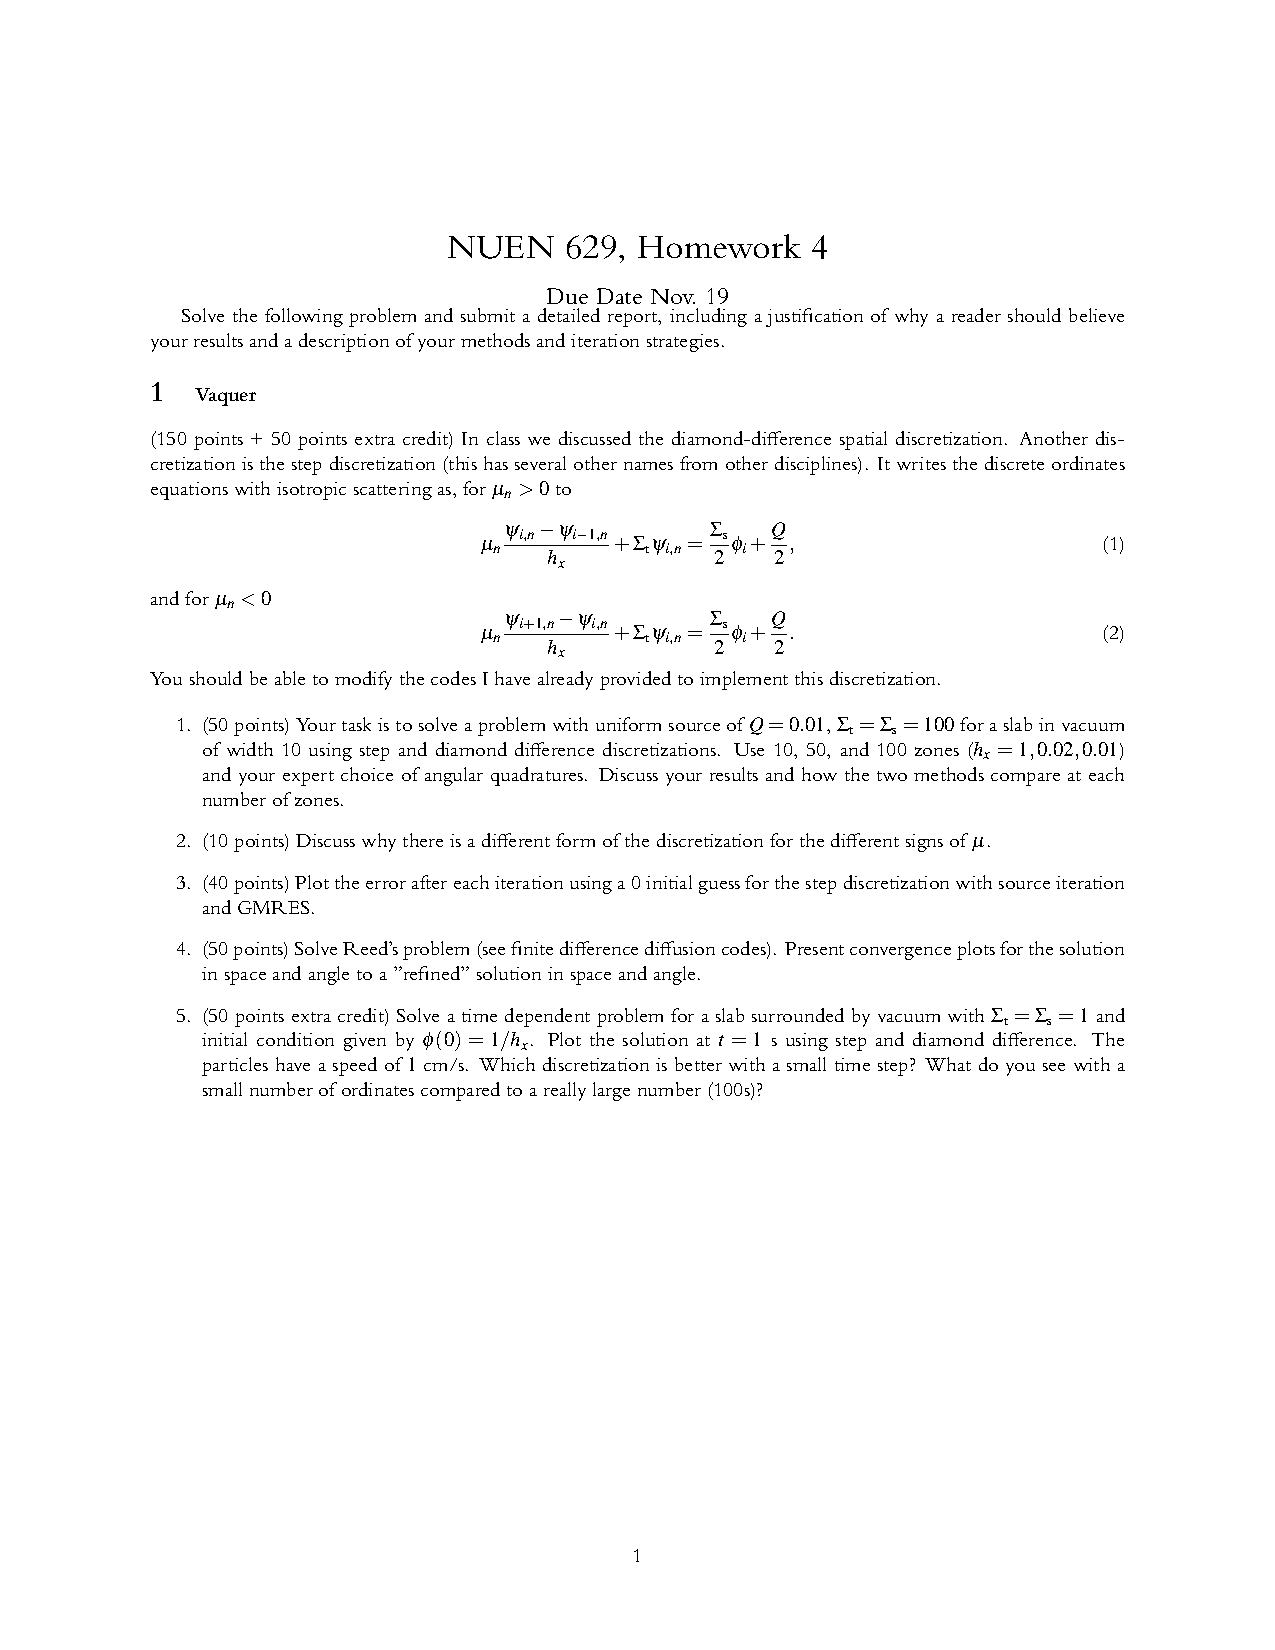
\includepdf{Homework4.pdf}

\begin{solnum}{1-1}

To modify the provided code to use the step discretization, essentially only the
1DSweep function needs to be modified.  For example, for a positive direction of
$\mu_n$ the flux in the $i$-th cell is, for the $k-th$ sweep,
\begin{equation}
    \psi^{(k+1)}_{i,n} = \frac{\frac{1}{2}\left(\phi^{(k)}_i + Q\right) +
    \frac{\mu_n}{h_x}\psi_{i-1,n}}{\Sigma_t + \frac{\mu_n}{h_x}},
\end{equation}
where $\psi_{i-1,n}$ is either defined by the boundary conditon, i.e., $\psi_{0} =
f(\mu_n)$, or is known from solution of the previous cell in the sweep. The negative
direction sweep is defined analogously. 

For the given problem parameters, source iteration was too slow to converge as $c=1$, so the
GMRES solver was used for both spatial discretizations.  This was verified to
converge to the same solution as source iteration for a sanity check.  A plot of the
different solutions for the different resolutions and spatial discretizations is
given below, for $N=16$ angles, in Fig.~\ref{fig1}. On
the finest mesh, increasing to $N=24$ had no visible effect on the solution.  The
solutions do not agree well between different refinements, or between step and the
diamond difference (DD) solutions.  The vast difference in solutions is due to the
large, pure scattering cross sections; neither step nor DD preserve the diffusion
limit.  Test problems with more modest cross sections ($\Sigma_t=1$ cm$^{-1}$, $c=0.5$)
showed good agreement as the mesh is refined, as shown in Fig.~\ref{fig2}

 Also plotted below is a finite difference diffusion 
solution to the same problem using Mark Boundary conditions for 100 cells, compared
to the step solution for 1000 cells.  It is
noted that for this problem diffusion theory should be fairly accurate, particularly
away from the boundaries.  Although the mesh for the transport solve is fine to the $O(1/\Sigma_t)$, the
solutions still seem to disagree.  This seems to be due to the fact that it is a pure
scattering solution. Although GMRES converges, there be some numerical stability
issues of some kind that cause the inaccuracy.  If we add a small amount of
absorption, with $\Sigma_t = \Sigma_s+0.001$, then the solutions agree much more
accurately on the interior.  

\begin{figure}[h!]
    \centering
    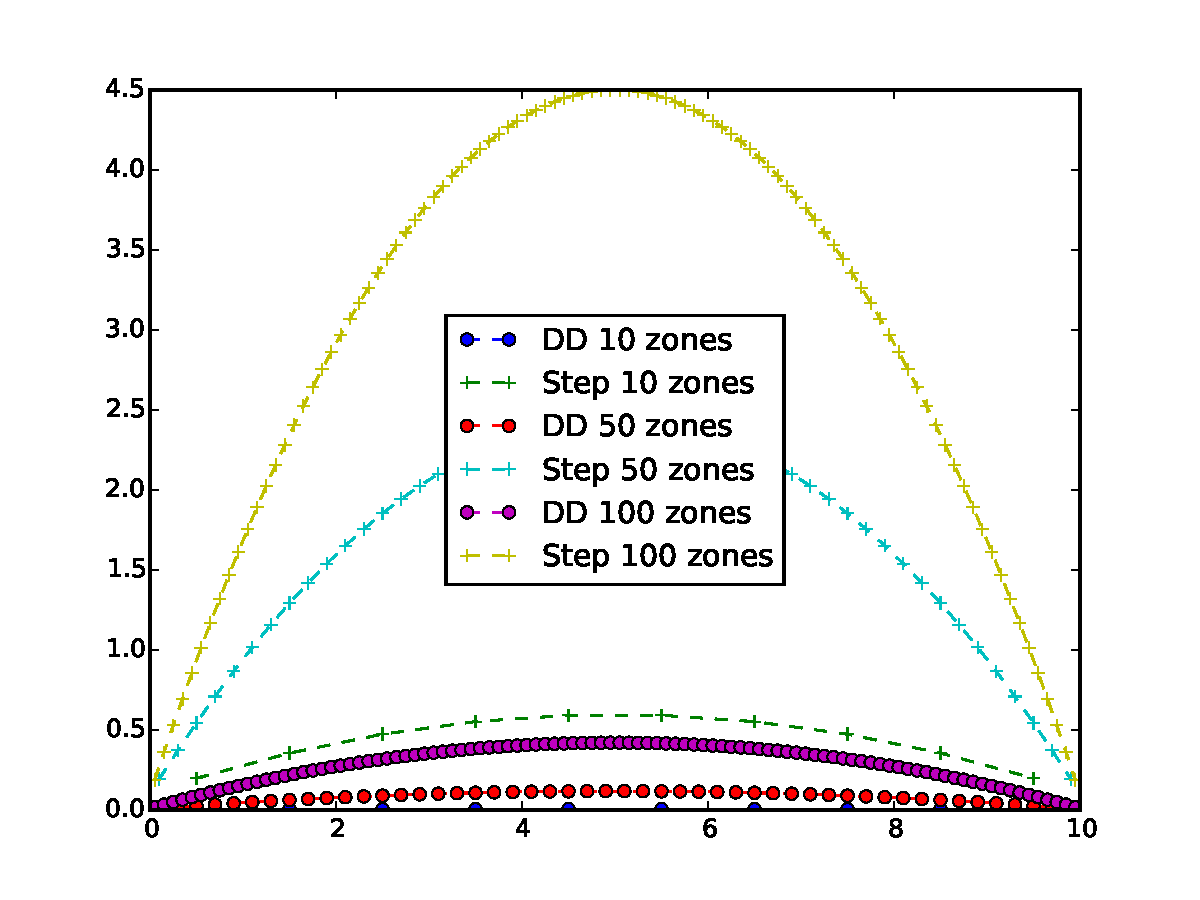
\includegraphics[width=0.5\textwidth]{prob1.pdf}
    \caption{Comparison of step and DD spatial discretizations for different numbers
        of zones.\label{fig1}}
\end{figure}
\begin{figure}[h!]
    \centering
    \includegraphics[width=0.5\textwidth]{prob1_thin.pdf}
    \caption{Comparison of step and DD spatial discretizations for different numbers
        of zones, with $\Sigma_s = \Sigma_a = 0.5$ cm$^{-1}$.\label{fig2}}
\end{figure}
\begin{figure}[h!]
    \centering
    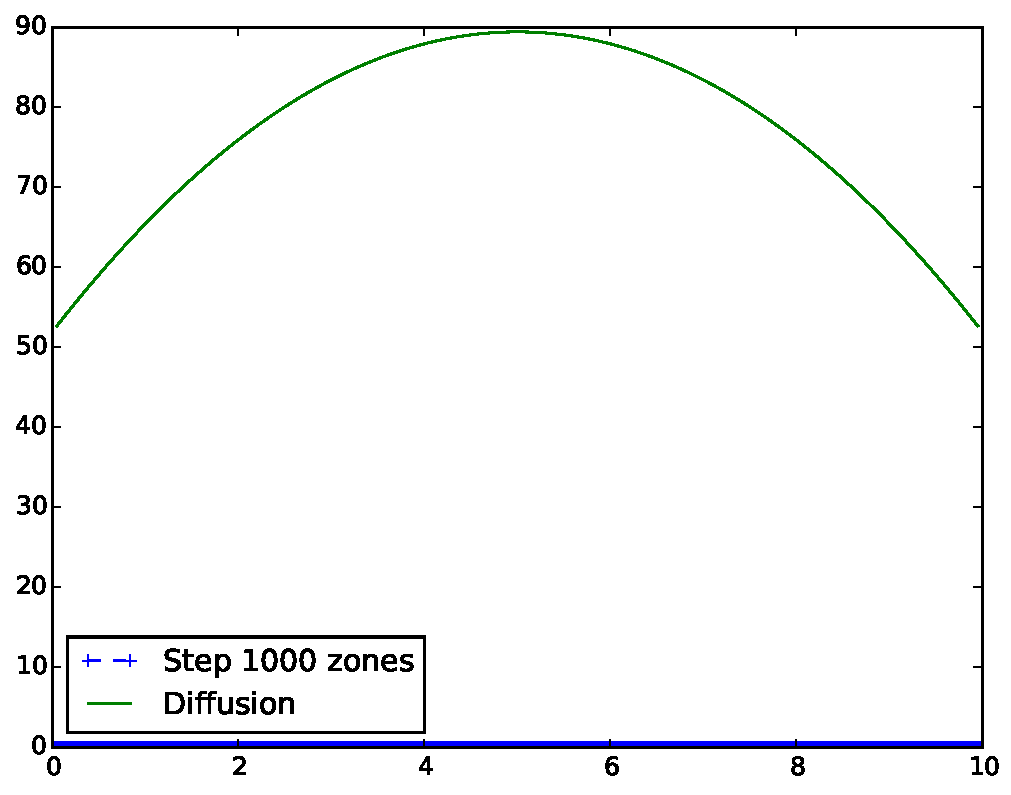
\includegraphics[width=0.5\textwidth]{diff.pdf}
    \caption{Comparison of diffusion and very fine mesh step solution.}
\end{figure}
\begin{figure}[h!]
    \cen
    

\end{solnum}

\begin{solnum}{1-2}

The different forms of the discretization are result of the solution being generally
undefined at the faces of cells, due to the discontinuity of the solution at cell
edges.  A closure of some kind must be defined because even in the weak-form we need
a value for $\psi$ on the face.  The given equations define $\psi$ on the face using the upwind closure, which attempts to numerically
propagate information in the physical direction of flow, based on the characteristic
flow of information in each direction.  This, in theory, resolves strong spatial
gradients with higher physical accuracy.  This closure also provides stability to the
equations, which could demonstrate oscillations with a poor choice of closure.

\end{solnum}

\begin{solnum}{1-3}



\end{solnum}

\clearpage

\clearpage
\subsubsection*{Code}
%\lstinputlisting[basicstyle=\scriptsize]{code.py}

\end{document}

